


\tikzset{every picture/.style={line width=0.75pt}} %set default line width to 0.75pt        

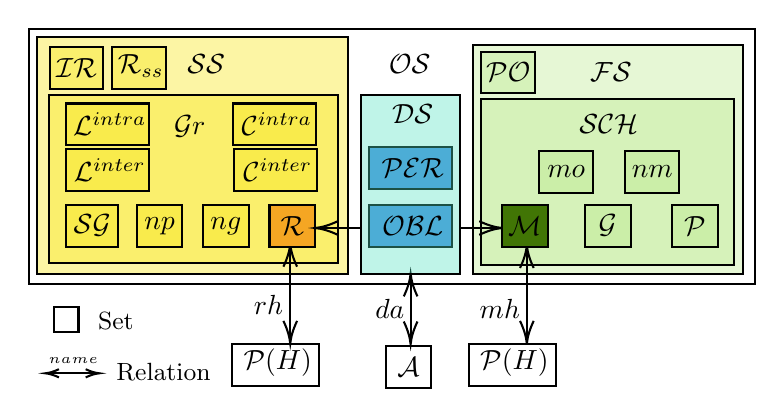
\begin{tikzpicture}[x=0.75pt,y=0.75pt,yscale=-1,xscale=1]
%uncomment if require: \path (0,2763); %set diagram left start at 0, and has height of 2763

%Shape: Rectangle [id:dp7560780738959927] 
\draw  [fill={rgb, 255:red, 255; green, 255; blue, 255 }  ,fill opacity=1 ] (140,1624) -- (490,1624) -- (490,1747) -- (140,1747) -- cycle ;
%Shape: Rectangle [id:dp8469798214550612] 
\draw  [fill={rgb, 255:red, 184; green, 233; blue, 134 }  ,fill opacity=0.34 ] (354,1632) -- (484,1632) -- (484,1742) -- (354,1742) -- cycle ;
%Shape: Rectangle [id:dp2847688578684602] 
\draw  [fill={rgb, 255:red, 184; green, 233; blue, 134 }  ,fill opacity=0.34 ] (358,1658) -- (480,1658) -- (480,1738) -- (358,1738) -- cycle ;
%Shape: Rectangle [id:dp46471880691149203] 
\draw  [fill={rgb, 255:red, 248; green, 231; blue, 28 }  ,fill opacity=0.4 ] (144,1628) -- (294,1628) -- (294,1742) -- (144,1742) -- cycle ;
%Straight Lines [id:da7210953862103895] 
\draw    (380,1730.31) -- (380,1773.69) ;
\draw [shift={(380,1775.69)}, rotate = 270] [color={rgb, 255:red, 0; green, 0; blue, 0 }  ][line width=0.75]    (10.93,-3.29) .. controls (6.95,-1.4) and (3.31,-0.3) .. (0,0) .. controls (3.31,0.3) and (6.95,1.4) .. (10.93,3.29)   ;
\draw [shift={(380,1728.31)}, rotate = 90] [color={rgb, 255:red, 0; green, 0; blue, 0 }  ][line width=0.75]    (10.93,-3.29) .. controls (6.95,-1.4) and (3.31,-0.3) .. (0,0) .. controls (3.31,0.3) and (6.95,1.4) .. (10.93,3.29)   ;
%Straight Lines [id:da9742405670873047] 
\draw    (348,1720) -- (366,1720) ;
\draw [shift={(368,1720)}, rotate = 180] [color={rgb, 255:red, 0; green, 0; blue, 0 }  ][line width=0.75]    (10.93,-3.29) .. controls (6.95,-1.4) and (3.31,-0.3) .. (0,0) .. controls (3.31,0.3) and (6.95,1.4) .. (10.93,3.29)   ;
%Shape: Rectangle [id:dp9760954045325634] 
\draw  [fill={rgb, 255:red, 248; green, 231; blue, 28 }  ,fill opacity=0.4 ] (149.56,1656) -- (289.06,1656) -- (289.06,1737) -- (149.56,1737) -- cycle ;
%Shape: Rectangle [id:dp6202366628126772] 
\draw  [fill={rgb, 255:red, 255; green, 255; blue, 255 }  ,fill opacity=1 ] (352,1776) -- (394,1776) -- (394,1796) -- (352,1796) -- cycle ;

%Shape: Rectangle [id:dp20067598884831228] 
\draw  [fill={rgb, 255:red, 248; green, 231; blue, 28 }  ,fill opacity=0.4 ] (192.06,1709) -- (214.06,1709) -- (214.06,1729) -- (192.06,1729) -- cycle ;

%Shape: Rectangle [id:dp006771319789144359] 
\draw  [fill={rgb, 255:red, 248; green, 231; blue, 28 }  ,fill opacity=0.4 ] (158.06,1709) -- (183.06,1709) -- (183.06,1729) -- (158.06,1729) -- cycle ;
%Shape: Rectangle [id:dp92237875722883] 
\draw  [fill={rgb, 255:red, 248; green, 231; blue, 28 }  ,fill opacity=0.4 ] (158.06,1682) -- (198.06,1682) -- (198.06,1702) -- (158.06,1702) -- cycle ;

%Shape: Rectangle [id:dp6591761395302378] 
\draw  [fill={rgb, 255:red, 248; green, 231; blue, 28 }  ,fill opacity=0.4 ] (158.06,1660) -- (198.06,1660) -- (198.06,1680) -- (158.06,1680) -- cycle ;

%Shape: Rectangle [id:dp11794703752595392] 
\draw  [fill={rgb, 255:red, 248; green, 231; blue, 28 }  ,fill opacity=0.4 ] (238.5,1660) -- (278.5,1660) -- (278.5,1680) -- (238.5,1680) -- cycle ;

%Shape: Rectangle [id:dp6557958558103134] 
\draw  [fill={rgb, 255:red, 248; green, 231; blue, 28 }  ,fill opacity=0.4 ] (239,1682) -- (279,1682) -- (279,1702) -- (239,1702) -- cycle ;

%Shape: Rectangle [id:dp8284992701408749] 
\draw  [fill={rgb, 255:red, 65; green, 117; blue, 5 }  ,fill opacity=1 ] (368,1709) -- (390,1709) -- (390,1729) -- (368,1729) -- cycle ;

%Shape: Rectangle [id:dp7066110016250453] 
\draw  [fill={rgb, 255:red, 248; green, 231; blue, 28 }  ,fill opacity=0.4 ] (224,1709) -- (246,1709) -- (246,1729) -- (224,1729) -- cycle ;

%Shape: Rectangle [id:dp4021333114319714] 
\draw  [fill={rgb, 255:red, 248; green, 231; blue, 28 }  ,fill opacity=0.4 ] (150.31,1633) -- (175.69,1633) -- (175.69,1653) -- (150.31,1653) -- cycle ;

%Shape: Rectangle [id:dp8476756388266236] 
\draw  [fill={rgb, 255:red, 248; green, 231; blue, 28 }  ,fill opacity=0.4 ] (180,1633) -- (206,1633) -- (206,1653) -- (180,1653) -- cycle ;

%Shape: Rectangle [id:dp07470576340681823] 
\draw  [fill={rgb, 255:red, 74; green, 144; blue, 226 }  ,fill opacity=1 ] (304,1681) -- (344,1681) -- (344,1701) -- (304,1701) -- cycle ;

%Shape: Rectangle [id:dp31407652093057714] 
\draw  [fill={rgb, 255:red, 74; green, 144; blue, 226 }  ,fill opacity=1 ] (304,1709) -- (344,1709) -- (344,1729) -- (304,1729) -- cycle ;

%Shape: Rectangle [id:dp053729126169398844] 
\draw  [fill={rgb, 255:red, 184; green, 233; blue, 134 }  ,fill opacity=0.34 ] (358,1635) -- (384,1635) -- (384,1655) -- (358,1655) -- cycle ;

%Shape: Rectangle [id:dp7720103442630182] 
\draw  [fill={rgb, 255:red, 184; green, 233; blue, 134 }  ,fill opacity=0.34 ] (385.94,1683) -- (411.94,1683) -- (411.94,1703) -- (385.94,1703) -- cycle ;

%Shape: Rectangle [id:dp3183552657000306] 
\draw  [fill={rgb, 255:red, 184; green, 233; blue, 134 }  ,fill opacity=0.34 ] (427.44,1683) -- (453.44,1683) -- (453.44,1703) -- (427.44,1703) -- cycle ;

%Shape: Rectangle [id:dp10802424702469593] 
\draw  [fill={rgb, 255:red, 184; green, 233; blue, 134 }  ,fill opacity=0.34 ] (408,1709) -- (430,1709) -- (430,1729) -- (408,1729) -- cycle ;

%Shape: Rectangle [id:dp16589412198505937] 
\draw  [fill={rgb, 255:red, 184; green, 233; blue, 134 }  ,fill opacity=0.34 ] (450,1709) -- (472,1709) -- (472,1729) -- (450,1729) -- cycle ;

%Shape: Rectangle [id:dp1270989692188249] 
\draw  [fill={rgb, 255:red, 255; green, 255; blue, 255 }  ,fill opacity=1 ] (238,1776) -- (280,1776) -- (280,1796) -- (238,1796) -- cycle ;

%Straight Lines [id:da8064666018529723] 
\draw    (266,1729.69) -- (266,1773.69) ;
\draw [shift={(266,1775.69)}, rotate = 270] [color={rgb, 255:red, 0; green, 0; blue, 0 }  ][line width=0.75]    (10.93,-3.29) .. controls (6.95,-1.4) and (3.31,-0.3) .. (0,0) .. controls (3.31,0.3) and (6.95,1.4) .. (10.93,3.29)   ;
\draw [shift={(266,1727.69)}, rotate = 90] [color={rgb, 255:red, 0; green, 0; blue, 0 }  ][line width=0.75]    (10.93,-3.29) .. controls (6.95,-1.4) and (3.31,-0.3) .. (0,0) .. controls (3.31,0.3) and (6.95,1.4) .. (10.93,3.29)   ;
%Shape: Rectangle [id:dp21027747628033966] 
\draw  [fill={rgb, 255:red, 245; green, 166; blue, 35 }  ,fill opacity=1 ] (256,1709) -- (278,1709) -- (278,1729) -- (256,1729) -- cycle ;

%Shape: Rectangle [id:dp8096748897019583] 
\draw  [fill={rgb, 255:red, 255; green, 255; blue, 255 }  ,fill opacity=1 ] (152,1758) -- (164,1758) -- (164,1770) -- (152,1770) -- cycle ;
%Straight Lines [id:da8952961464283278] 
\draw    (150,1790) -- (172,1790) ;
\draw [shift={(174,1790)}, rotate = 180] [color={rgb, 255:red, 0; green, 0; blue, 0 }  ][line width=0.75]    (6.56,-1.97) .. controls (4.17,-0.84) and (1.99,-0.18) .. (0,0) .. controls (1.99,0.18) and (4.17,0.84) .. (6.56,1.97)   ;
\draw [shift={(148,1790)}, rotate = 0] [color={rgb, 255:red, 0; green, 0; blue, 0 }  ][line width=0.75]    (6.56,-1.97) .. controls (4.17,-0.84) and (1.99,-0.18) .. (0,0) .. controls (1.99,0.18) and (4.17,0.84) .. (6.56,1.97)   ;
%Shape: Rectangle [id:dp07012270906311535] 
\draw  [fill={rgb, 255:red, 255; green, 255; blue, 255 }  ,fill opacity=1 ] (312,1777) -- (334,1777) -- (334,1797) -- (312,1797) -- cycle ;

%Straight Lines [id:da5115868277627034] 
\draw    (324,1744) -- (324,1774) ;
\draw [shift={(324,1776)}, rotate = 270] [color={rgb, 255:red, 0; green, 0; blue, 0 }  ][line width=0.75]    (10.93,-3.29) .. controls (6.95,-1.4) and (3.31,-0.3) .. (0,0) .. controls (3.31,0.3) and (6.95,1.4) .. (10.93,3.29)   ;
\draw [shift={(324,1742)}, rotate = 90] [color={rgb, 255:red, 0; green, 0; blue, 0 }  ][line width=0.75]    (10.93,-3.29) .. controls (6.95,-1.4) and (3.31,-0.3) .. (0,0) .. controls (3.31,0.3) and (6.95,1.4) .. (10.93,3.29)   ;
%Straight Lines [id:da05763610491020765] 
\draw    (300,1720) -- (280,1720) ;
\draw [shift={(278,1720)}, rotate = 360] [color={rgb, 255:red, 0; green, 0; blue, 0 }  ][line width=0.75]    (10.93,-3.29) .. controls (6.95,-1.4) and (3.31,-0.3) .. (0,0) .. controls (3.31,0.3) and (6.95,1.4) .. (10.93,3.29)   ;
%Shape: Rectangle [id:dp4122292872961708] 
\draw  [fill={rgb, 255:red, 80; green, 227; blue, 194 }  ,fill opacity=0.36 ] (300,1656) -- (348,1656) -- (348,1742) -- (300,1742) -- cycle ;

% Text Node
\draw (161.5,1784) node  [font=\tiny] [align=left] {$name$};
% Text Node
\draw (314,1759) node   [align=left] {$da$};

% Text Node
\draw (202,1787) node  [font=\footnotesize] [align=left] 
{\begin{minipage}[lt]{29.67pt}\setlength\topsep{0pt}
\begin{center}
{\small Relation}
\end{center}
\end{minipage}};

% Text Node
\draw (182,1765) node  [font=\footnotesize] [align=left] {\begin{minipage}[lt]{13.75pt}\setlength\topsep{0pt}
\begin{center}
{\small Set}
\end{center}

\end{minipage}};
% Text Node
\draw (323.5,1641) node   [align=left] {$\mathcal{OS}$};
% Text Node
\draw (170.56,1719) node   [align=left] {$\mathcal{SG}$};
% Text Node
\draw (325,1665) node   [align=left] {$\mathcal{DS}$};
% Text Node
\draw (225.5,1641) node   [align=left] {$\mathcal{SS}$};
% Text Node
\draw (367,1759) node   [align=left] {$mh$};
% Text Node
\draw (255.5,1757) node   [align=left] {$rh$};
% Text Node
\draw (217.56,1671) node   [align=left] {$\mathcal{G}r$};
% Text Node
\draw (420.5,1645) node   [align=left] {$\mathcal{FS}$};
% Text Node
\draw (419.44,1670) node   [align=left] {$\mathcal{SCH}$};
% Text Node
\draw (323,1787) node   [align=left] {$\mathcal{A}$};
% Text Node
\draw (267,1719) node   [align=left] {$\mathcal{R}$};
% Text Node
\draw (260,1785) node   [align=left] {$\mathcal{P}(H)$};
% Text Node
\draw (461,1719) node   [align=left] {$\mathcal{P}$};
% Text Node
\draw (419,1719) node   [align=left] {$\mathcal{G}$};
% Text Node
\draw (440.44,1693) node   [align=left] {$nm$};
% Text Node
\draw (398.94,1693) node   [align=left] {$mo$};
% Text Node
\draw (371,1645) node   [align=left] {$\mathcal{PO}$};
% Text Node
\draw (325,1719) node   [align=left] {$\mathcal{OBL}$};
% Text Node
\draw (325,1691) node   [align=left] {$\mathcal{PER}$};
% Text Node
\draw (194,1642) node   [align=left] {$\mathcal{R}_{ss}$};
% Text Node
\draw (163,1643) node   [align=left] {$\mathcal{IR}$};
% Text Node
\draw (235,1719) node   [align=left] {$ng$};
% Text Node
\draw (379,1719) node   [align=left] {$\mathcal{M}$};
% Text Node
\draw (260,1692) node   [align=left] {$\mathcal{C}^{inter}$};
% Text Node
\draw (259.5,1670) node   [align=left] {$\mathcal{C}^{intra}$};
% Text Node
\draw (179.06,1670) node   [align=left] {$\mathcal{L}^{intra}$};
% Text Node
\draw (179.06,1692) node   [align=left] {$\mathcal{L}^{inter}$};
% Text Node
\draw (203.06,1719) node   [align=left] {$np$};
% Text Node
\draw (374,1785) node   [align=left] {$ \mathcal{P}(H)$};


\end{tikzpicture}